\documentclass[12pt, letterpaper, titlepage]{article}
\usepackage[utf8]{inputenc}
\usepackage{geometry}
\usepackage{color,graphicx,overpic} 
\usepackage{fancyhdr}
\usepackage{amsmath,amsthm,amsfonts,amssymb}
\usepackage{mathtools}
\usepackage{hyperref}
\usepackage{multicol}
\usepackage{float}
\usepackage{blindtext}
\usepackage{longtable}
\usepackage{scrextend}
\usepackage[font=small,labelfont=bf]{caption}
\usepackage{calc}
\usepackage{titlesec}
\usepackage{listings}
\usepackage[normalem]{ulem}
\usepackage{tabularx}
\usepackage{mathrsfs}
\usepackage{bookmark}
\usepackage{apple_emoji}
\usepackage{setspace}
\usepackage{ragged2e}
\usepackage{ltablex}
\usepackage{xurl}
\usepackage{tikz}
\usepackage{pgfplots}
\usepackage{xparse}

\mathtoolsset{showonlyrefs}  
\allowdisplaybreaks
\lstset{basicstyle=\ttfamily, keywordstyle=\rmfamily\bfseries}

\definecolor{comment}{RGB}{140, 140, 140}
\definecolor{text}{RGB}{0, 0, 0}
\definecolor{string}{rgb}{0.58,0,0}
\definecolor{variable}{RGB}{244, 63, 78}

\lstdefinestyle{code_style}{
    commentstyle=\color{comment},
    keywordstyle=\color{variable},
    numberstyle=\tiny\color{text},
    stringstyle=\color{string},
    basicstyle=\ttfamily\scriptsize\color{text},
    breakatwhitespace=false,         
    breaklines=true,                 
    captionpos=b,                    
    keepspaces=true,                 
    numbers=left,                    
    numbersep=-10pt,                  
    showspaces=false,                
    showstringspaces=false,
    showtabs=false,                  
    tabsize=4
}

\newcolumntype{q}{>{\hsize=.45\hsize}X}
\newcolumntype{e}{>{\hsize=.35\hsize}X}
\newcolumntype{s}{>{\hsize=.15\hsize}X}

\definecolor{mycolor}{rgb}{0, 0, 0}

\geometry{top=2.54cm, left=2.54cm, right=2.54cm, bottom=2.54cm}
\setlength{\headheight}{20pt}
\setlength{\parskip}{0.5cm}
\setlength{\parindent}{0.5cm}

\pgfplotsset{width=\textwidth-3cm,compat=newest}
\usepgfplotslibrary{patchplots}
\renewcommand{\thesection}{} % Make sections have no number

\newcommand{\B}{
\includegraphics[height=1.5em, valign=B, raise=-0.2em]{BigB.png}} 
\newcommand{\nx}{$n\times1$}

\title{\textbf{\Huge{
    \begin{center}
        ECE 322 Lab Report \#4
    \end{center}
}}}
\author{
\B enjamin Kong \\
1573684 \\
}

\pagestyle{fancy}
\fancyhf{}
\rhead{\thepage}
\lhead{\textit{ECE 322 Lab Report \#4}}

\begin{document} 
\onehalfspacing

\maketitle
\newpage

\section*{Introduction}
The purpose of this lab was to introduce integration white box testing techniques. We will use Python and Python unittest unittest.mock to gain experience with integration testing.

Integration testing is the logical extension of unit testing. There are two common approaches:
\begin{itemize}
    \item Non-incremental testing (big bang): where each module is tested independently, then the system is tested as a whole, and
    \item Incremental testing: where the set of previously tested modules are combined with the next module to be tested before running tests. There are two common methods of incremental testing:
    \begin{itemize}
        \item Bottom up: where the lowest level modules are tested in isolation, then higher level modules are added incrementally, and
        \item Top down: where the highest level modules are tested in isolation (stubbing lower level modules), then lower level modules are added incrementally.
    \end{itemize}
\end{itemize}

Usually, when integration testing is performed, we need to use stubs and drivers. In this lab, we will be creating mock objects which are essentially used as stubs in our integration tests.
\begin{itemize}
    \item Stubs are used as a stand in for lower level modules that aren't currently being tested. Stubs return dummy values or makes an assertion so that the higher level modules can still run and be tested.
    \item Drivers are a piece of testing code that make it possible to call the submodule of an application by itself. Often, driver code requires stub setup and object initialization. 
\end{itemize}

We will be testing a simple database system that has seven modules, Module A to module F. We will be focusing on non-incremental testing (big bang integration).

\section*{Task}
For this lab, we tested the database application using the big bang testing technique. We created unit tests for each module A-F. Any time a module depended on another module, we mocked that module. The code for the tests have been included with the submission under \lstinline{Lab4_src/tests}. The table of tests and results is displayed below.

\footnotesize
\begin{centering}
\begin{tabularx}{\textwidth}{|q|X|q|e|e|X|e|}
    \caption{Test cases for \lstinline{bisect.py}} \\ \hline
    \textbf{Test ID} & \textbf{Description} & \textbf{func} & \textbf{x1} & \textbf{x2} & \textbf{Expected} & \textbf{Pass} \\ \hline
    1 & Normal case & $x + 1$ & -10 & 10 & 0 & Y \\ \hline
\end{tabularx}
\end{centering}
\normalsize

An image of the coverage report is provided below.
\begin{figure}[H]
    \caption{Coverage report of \lstinline{mybisect.py}. The only relevant value has been marked with a red arrow.}
    % 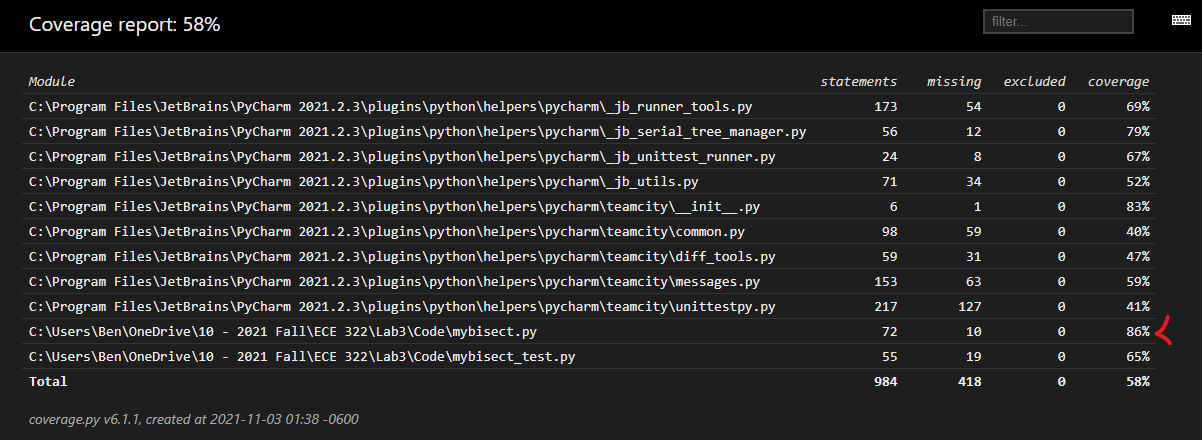
\includegraphics[width=\textwidth]{CodeCoverage1.png}
    \centering
\end{figure}

\section*{Conclusion}
The purpose of this lab was to introduce integration white box testing techniques. We used Python and Python unittest unittest.mock to gain experience with integration testing.

Integration testing is the logical extension of unit testing. There are two common approaches: non-incremental testing (big bang) where each module is tested independently, then the system is tested as a whole, and incremental testing where the set of previously tested modules are combined with the next module to be tested before running tests. There are two common methods of incremental testing: Bottom up where the lowest level modules are tested in isolation, then higher level modules are added incrementally, and top down where the highest level modules are tested in isolation (stubbing lower level modules), then lower level modules are added incrementally.

Usually, when integration testing is performed, we need to use stubs and drivers. In this lab, we created mock objects which are essentially used as stubs in our integration tests. Stubs are used as a stand in for lower level modules that aren't currently being tested. Stubs return dummy values or makes an assertion so that the higher level modules can still run and be tested. Drivers are a piece of testing code that make it possible to call the submodule of an application by itself. Often, driver code requires stub setup and object initialization. 

In the lab, we tested a simple database system that had seven modules, Module A to module F. We focused on non-incremental testing (big bang integration).

\end{document}
